\subsubsection{Random Data Creation}
\label{mock-data}
To evaluate WolfTutor without bias, random mock tutors were 
created via functions from python's Random library, except for
tutoring subjects as all tutors could tutor in the four possible subjects,
names which were generated as User N where N was the number of the 
user in creation order, and emails being userN@ncsu.edu. Two 
separate databases were created for both the new WolfTutor application
and the old, to prevent reviewers from automatically looking for a tutor
they liked when moving from one application to another.

Originally, majors and degree level were chosen randomly, but
during in person evaluations, many reviewers voiced that they did not
see what they were looking for in a tutor. For example, one reviewer specifically wanted
a Computer Science major with an extremely high GPA but the highest GPAs 
belonged to other majors. Another reviwer wanted only tutors with Master degrees
and felt that they did not have many options. For the second day of 
evaluations, instead of creating more options, new databases were created such that all majors
were Computer Science and all degrees were Masters. Adding more options
would have created more load than the application was currently able to handle.
The second day reviwers were noticeably more content and less confused.


\subsubsection{Random Data Distributions}

\begin{figure}[t]
\caption{GPA Distribution with 1000 Tutors}
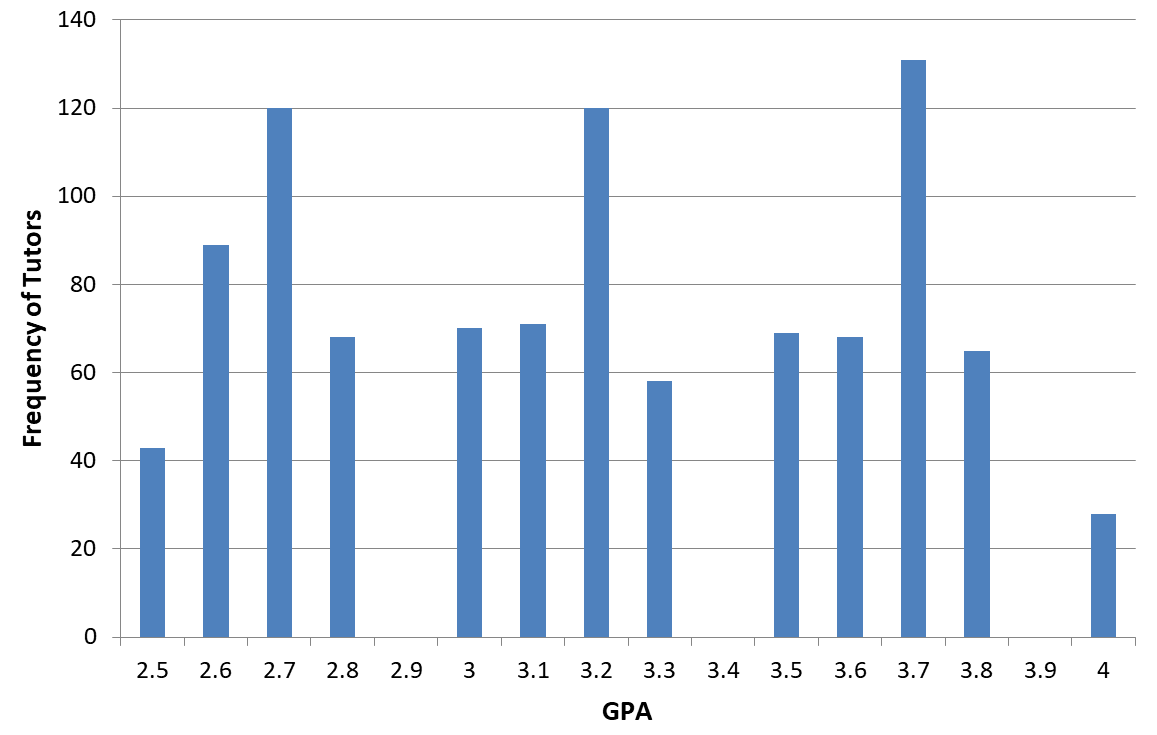
\includegraphics[width=0.5\textwidth]{gpa_test1.png}
\label{fig:gpa}
\end{figure}

\begin{figure}[t]
\caption{Average Review Score Distribution with 1000 Tutors}
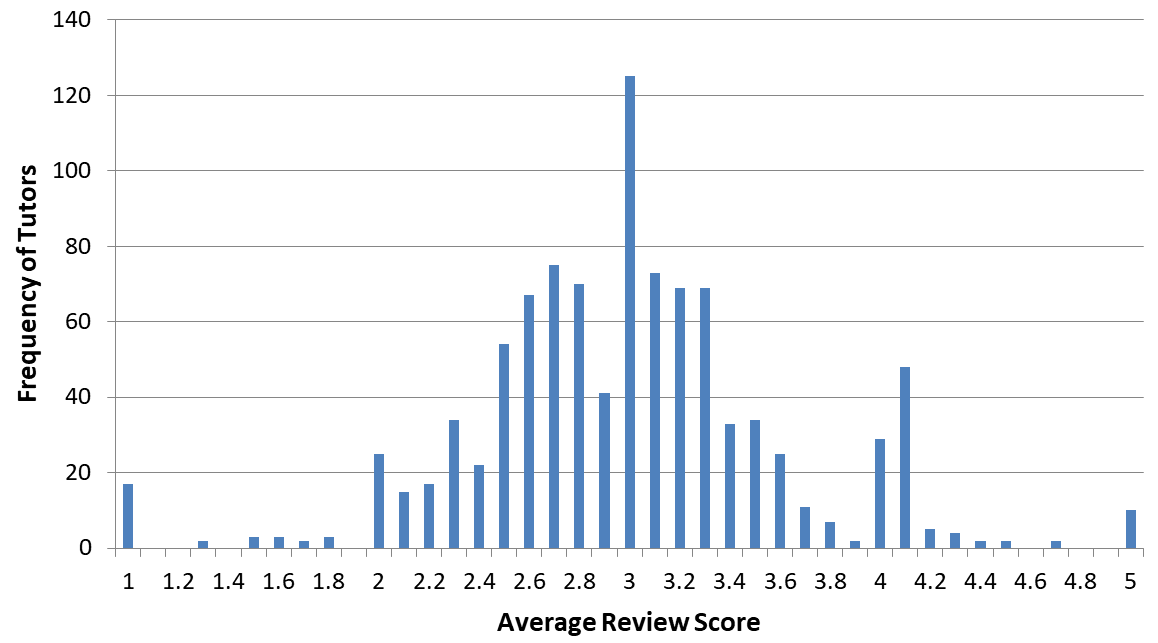
\includegraphics[width=0.5\textwidth]{scores_test1.png}
\label{fig:scores}
\end{figure}

During day 1 in person evaluations, it was noted that there
seemed to be one or two 'God' tutors that were popular. With
further inspection, it was determined that the database was a bit
too random and needed to be altered slightly to avoid a situation where a 
small number of tutors were obviously better than the others in order
to better test the time needed to use the application more realistically.
For example, not allowing the tutor with the highest GPA to also have the
best average review score.

This issue was investigated by creating histograms for the distributions
of both GPA and average review score over 1000 tutors. Figure \ref{fig:gpa} 
is the distribution of GPAs created for one test. Additional tests created nearly
identical distributions. Figure \ref{fig:scores} is the distribution of average
review scores for one test. Additional tests created nearly identical distributions
in this case as well. 

The GPA distribution is discrete uniform as it should be. However, tutor GPA is not
best represented as uniform because if someone has a very low GPA, they
likely don't know enough about the subject to tutor it. Students also typically don't
want a tutor with a bad GPA. Because of this, some GPAs between 1.0 and 2.0 were 
raised to between 3.0 and 4.0 for day 2 evaluations. 

The average review score distribution is not uniform because it is calculated by
taking the average of the individual scores given generated as discrete uniform 
distribution. Taking the average created an almost normal distribution. This seemed
to work well for day 1 evaluations, however, some alterations were made to the day 2
database to create more competition between the tutors and to avoid 'God' tutors previously
mentioned. 





